\documentclass[]{beamer}
\usetheme{Dresden}
% \useoutertheme{split}

\usepackage{color}
\usepackage{graphicx}
\usepackage{listings}
\usepackage{lmodern} %% allow bold keywords
\usepackage{menukeys}
\usepackage{qtree}

\definecolor{darkgreen}{rgb}{0,0.5,0}
\definecolor{lightblue}{rgb}{0.2,0.2,1}

\lstset{language=Java,
	basicstyle=\ttfamily\footnotesize,
	keywordstyle=\color{purple},
	commentstyle=\color{darkgreen},
	numberstyle=\tiny\color{gray},
	stringstyle=\color{blue},
	tabsize=4,
	showstringspaces=false,
	breaklines=true,
	keepspaces=true,
	numbers=left,
	escapechar=@
}

\title{Java}
\subtitle{Javadoc}
\author{FSR Informatik}
\date{\today}

\begin{document}

\begin{frame}
\titlepage
\end{frame}
\begin{frame}{Overview}
\tableofcontents
\end{frame}

\section{Javadoc}
\subsection{Overview}
\begin{frame}{}
	Javadoc creates a HTML documentation from your code.
	\vfill
	Structured comments with annotations are used as source.
\end{frame}

\begin{frame}{Eclipse}
	To create the Javadoc for your current project: \\
	\menu[,]{Project, Generate Javadoc\dots}
	\vfill
	Make sure you had installed Javadoc. 
	If not the \keys{Finish} button will stay grey.
\end{frame}

\subsection{Annotations}
\begin{frame}[fragile]{Class}
	An example class without methods:
	\begin{lstlisting}[basicstyle=\ttfamily\scriptsize, escapechar=!,
	commentstyle=\color{lightblue}]
    import java.util.List;

    /**
     * A bookshelf stores an unlimited amount of books.
     * @author Jane Doe
     *
     */
    public class Bookshelf {
    
	    private List<Book> books;

    }
	\end{lstlisting}
\end{frame}

\begin{frame}{Class}
	You see the description of the class from the previous slide.
	\vfill
	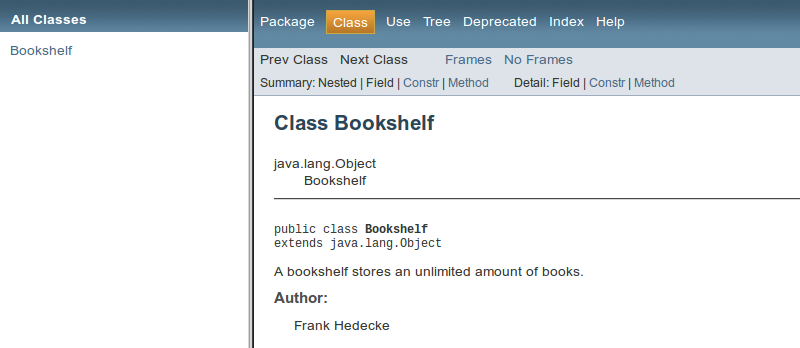
\includegraphics[scale=0.3]{res/javadoc_class.png}
\end{frame}

\begin{frame}[fragile]{Method}
	Add a small description of your method.
	\begin{lstlisting}[basicstyle=\ttfamily\scriptsize, escapechar=!,
	commentstyle=\color{lightblue}]
	/**
	 * A Constructor for Bookshelf.
	 */
	public Bookshelf() {
	    books = new LinkedList<Book>();
	}
	\end{lstlisting}
\end{frame}

\begin{frame}[fragile]{Method with Parameter}
	Use \textbf{@param} to describe every parameter
	\begin{lstlisting}[basicstyle=\ttfamily\scriptsize, escapechar=!,
	commentstyle=\color{lightblue}]
	/**
	 * Puts a book into the bookshelf.
	 * @param book that will be added in the bookshelf
	 */
	public void addBook(Book book) {
	    this.books.add(book);
	}
	\end{lstlisting}
\end{frame}

\begin{frame}[fragile]{Method with Return Value}
	Use \textbf{@return} to describe the return value.
	\begin{lstlisting}[basicstyle=\ttfamily\scriptsize, escapechar=!,
	commentstyle=\color{lightblue}]
	/**
	 * Returns the number of stored books.
	 * @return number of stored books
	 */
	public int countBooks() {
	    return books.size();
	}
	\end{lstlisting}
	\vfill
\end{frame}

\begin{frame}[fragile]{Method with Parameter and Return Value}
	For boolean: Describe in which case a method returns true.
	\begin{lstlisting}[basicstyle=\ttfamily\scriptsize, escapechar=!,
	commentstyle=\color{lightblue}]
	/**
	 * Checks if shelf contains a specific book.
	 * @param book whose occurrence is checked
	 * @return true if the shelf contains the given book
	 */
	public boolean containsBook(Book book) {
	    return books.contains(book);
	}
	\end{lstlisting}
\end{frame}

\subsection{More on Javadoc}
\begin{frame}
	Javadoc shows a summary of all methods and constructors. \\
	A detailed view is below the summary.
	\vfill
	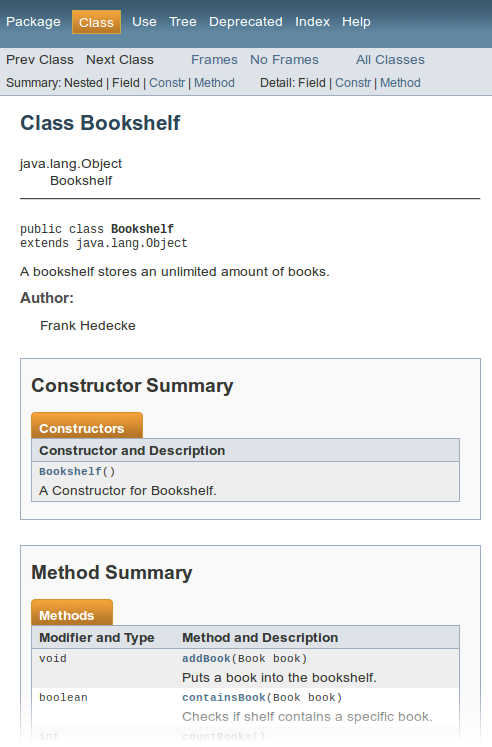
\includegraphics[scale=0.25]{res/javadoc_shelf_left.png}
	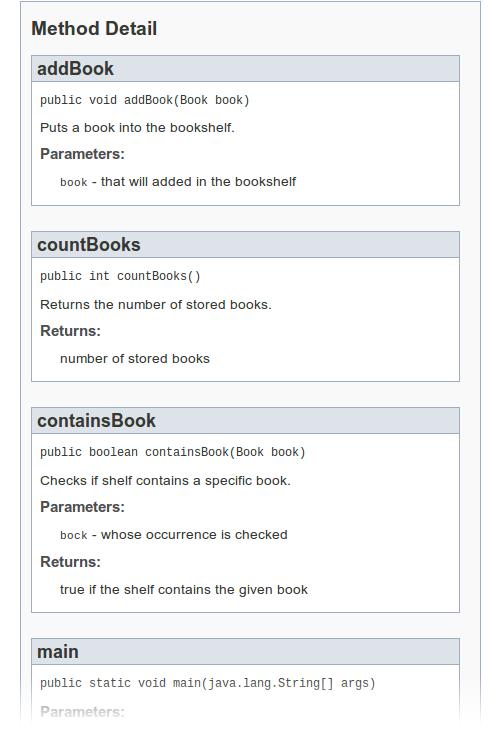
\includegraphics[scale=0.25]{res/javadoc_shelf_right.png}
\end{frame}

\begin{frame}{Eclipse Tooltips}
	Hovering a method opens a tooltip displaying information like in the Javadoc.
	\vfill
	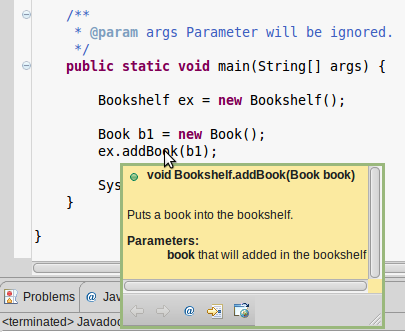
\includegraphics[scale=0.35]{res/javadoc_eclipse.png}
\end{frame}

\begin{frame}[fragile]{Example - A second Class}
	Another class.
	\begin{lstlisting}[basicstyle=\ttfamily\scriptsize, escapechar=!,
	commentstyle=\color{lightblue}]
	/**
	 * A book.
	 * @author John Doe
	 *
	 */
	public class Book {

	}
	\end{lstlisting}
\end{frame}

\begin{frame}[fragile]{More classes}
	After pressing \menu[,]{Project, Generate Javadoc\dots}
	you can choose which classes shall be included.
	\vfill
	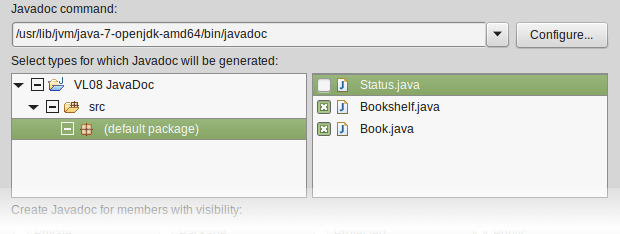
\includegraphics[scale=0.35]{res/javadoc_selection.png}
	\vfill
	The left view shows a tree with all packages. 
	After selecting a package you can select your classes.
\end{frame}

\begin{frame}[fragile]{More classes}
	Now you see both selected classes in the Javadoc.
	\vfill
	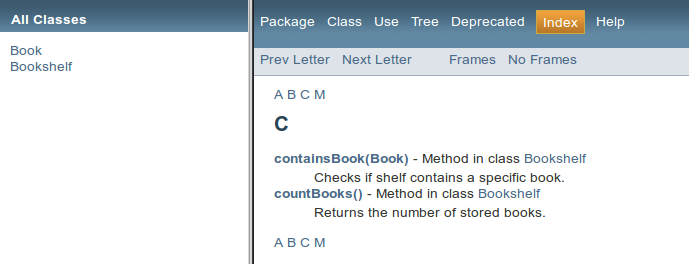
\includegraphics[scale=0.35]{res/javadoc_multiple_classes.png}
	\vfill
	The view \emph{Index} shows a list of all methods, constructors, \dots
\end{frame}

\section{Lost Stuff}
\subsection{}
\begin{frame}[fragile]{Constructors with this}
	Remember: \textbf{this} is a reference to the current object.
	\vfill
	\textbf{this()} calls the constructor. 
	So you can write multiple constructors with less code.
	\begin{lstlisting}
	public class Example {
	
	    public String value;
	
	    Example(String value) {
	        this.value = value;
	    }
	
	    Example() {
	        this("standard");	    
	    }
	}
	\end{lstlisting}
\end{frame}

\begin{frame}[fragile]{Extended use of super}
	In the previous lectures we used \textbf{super()} to call the constructor from the superclass.
	We can use \textbf{super} to call any other method from the superclass.
	\begin{lstlisting}[escapechar=!]
	import java.util.*;

	public class StringSet extends HashSet<String> {
	
	    @Override
	    public boolean add(String elem) {
	        // add a "?" to every String added to this set
	        return super.add(elem + "?");
	    }
	}
	\end{lstlisting}
\end{frame}

\begin{frame}[fragile]{Return for Void Methods}
	Void methods can have a return statement, too. 
	The empty return statement stops the execution of the method early.
	\begin{lstlisting}
	public void foo (boolean condition, int x) {
	
	    if (condition) {
	        return;
	    }
	    
	    for (int i = 1; i <= x; i++) {
	        System.out.println(i);
	    }
	}
	\end{lstlisting}
\end{frame}

\end{document}